\documentclass[border=10pt]{standalone}
\usepackage{tikz}
\usetikzlibrary{shapes,arrows,positioning,calc,decorations.pathmorphing}
\usepackage{fontspec}
\setmainfont{DejaVu Sans}

% Styles pour les équipements réseau
\tikzstyle{router} = [rectangle, draw=blue!50, fill=blue!20, thick, minimum width=2cm, minimum height=1.5cm, text centered, text width=2cm]
\tikzstyle{switch} = [rectangle, draw=green!50, fill=green!20, thick, minimum width=1.5cm, minimum height=1cm, text centered]
\tikzstyle{server} = [rectangle, draw=red!50, fill=red!20, thick, minimum width=1.5cm, minimum height=1cm, text centered]
\tikzstyle{client} = [rectangle, draw=orange!50, fill=orange!20, thick, minimum width=1cm, minimum height=0.8cm, text centered]
\tikzstyle{cloud} = [ellipse, draw=gray!50, fill=gray!20, thick, minimum width=3cm, minimum height=2cm, text centered]

\begin{document}
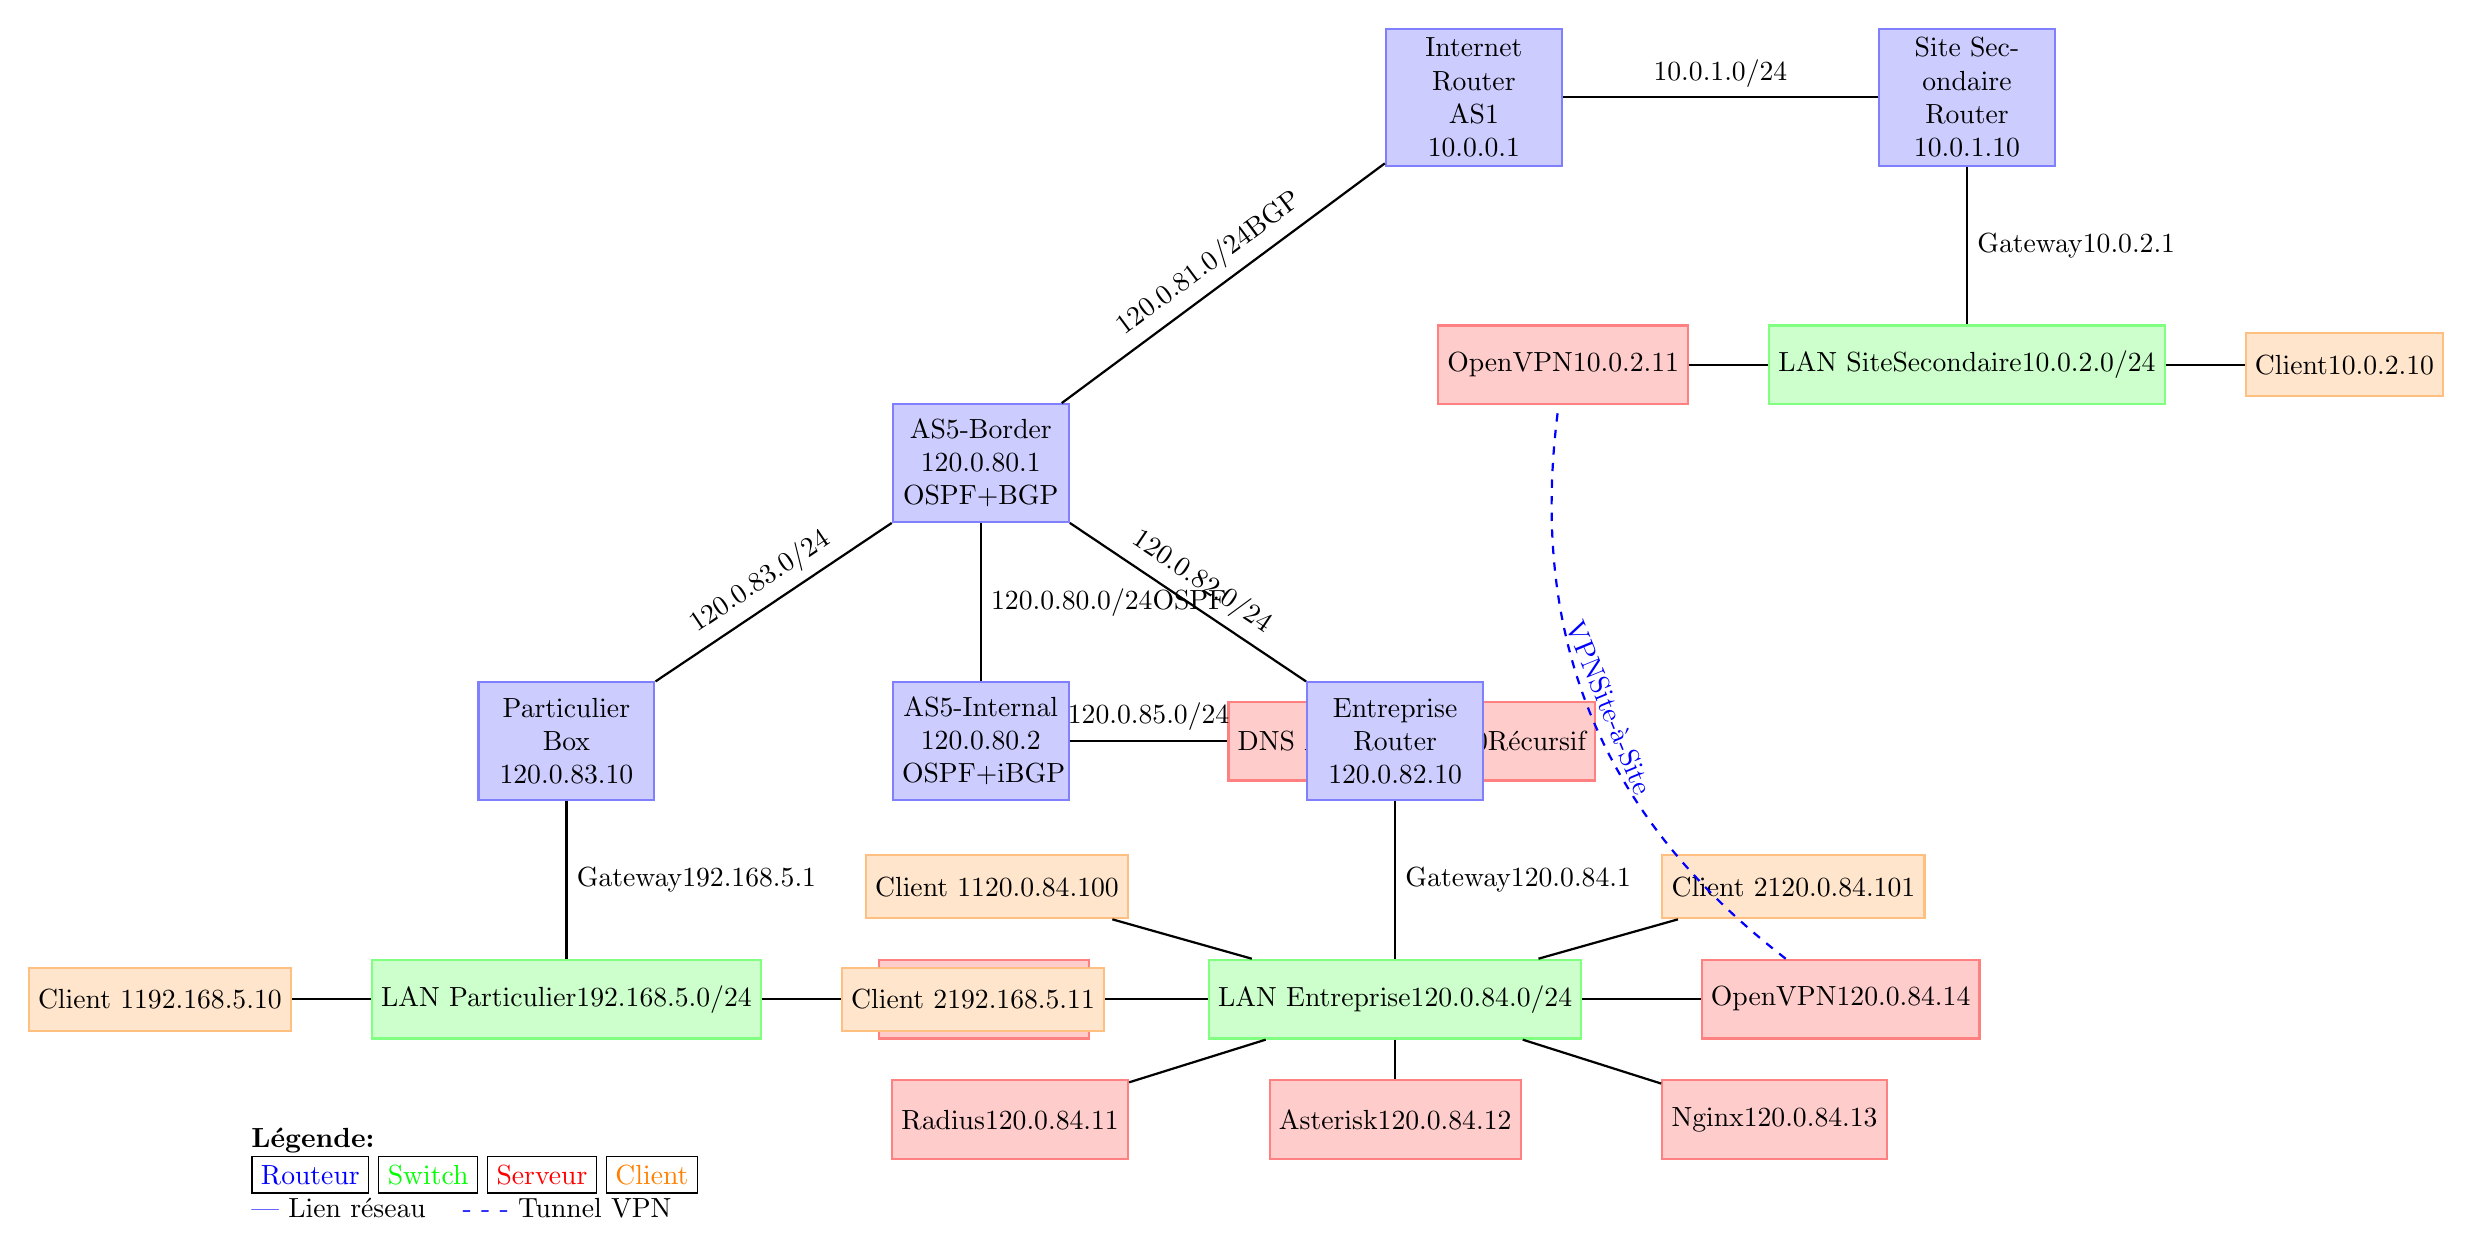
\begin{tikzpicture}[node distance=2cm, auto]

% Internet Router (AS1)
\node[router] (internet) {Internet Router\\AS1\\10.0.0.1};

% AS5-Border Router
\node[router, below left=3cm and 4cm of internet] (as5border) {AS5-Border\\120.0.80.1\\OSPF+BGP};

% AS5-Internal Router
\node[router, below=2cm of as5border] (as5internal) {AS5-Internal\\120.0.80.2\\OSPF+iBGP};

% Internet Router - AS5 Border link
\draw[thick] (internet) -- node[above, sloped] {120.0.81.0/24\\BGP} (as5border);

% AS5 Border - AS5 Internal link
\draw[thick] (as5border) -- node[right] {120.0.80.0/24\\OSPF} (as5internal);

% Services AS5
\node[server, right=2cm of as5internal] (dnsas5) {DNS AS5\\120.0.85.10\\Récursif};
\draw[thick] (as5internal) -- node[above] {120.0.85.0/24} (dnsas5);

% Entreprise Router
\node[router, below right=2cm and 3cm of as5border] (entrouter) {Entreprise\\Router\\120.0.82.10};
\draw[thick] (as5border) -- node[above, sloped] {120.0.82.0/24} (entrouter);

% LAN Entreprise
\node[switch, below=2cm of entrouter] (entlan) {LAN Entreprise\\120.0.84.0/24};
\draw[thick] (entrouter) -- node[right] {Gateway\\120.0.84.1} (entlan);

% Services Entreprise
\node[server, left=1.5cm of entlan] (dnsent) {DNS\\120.0.84.10};
\node[server, below left=0.5cm and 1cm of entlan] (radius) {Radius\\120.0.84.11};
\node[server, below=0.5cm of entlan] (asterisk) {Asterisk\\120.0.84.12};
\node[server, below right=0.5cm and 1cm of entlan] (nginx) {Nginx\\120.0.84.13};
\node[server, right=1.5cm of entlan] (openvpn) {OpenVPN\\120.0.84.14};

\draw[thick] (entlan) -- (dnsent);
\draw[thick] (entlan) -- (radius);
\draw[thick] (entlan) -- (asterisk);
\draw[thick] (entlan) -- (nginx);
\draw[thick] (entlan) -- (openvpn);

% Clients Entreprise
\node[client, above left=0.5cm and 1cm of entlan] (client1) {Client 1\\120.0.84.100};
\node[client, above right=0.5cm and 1cm of entlan] (client2) {Client 2\\120.0.84.101};
\draw[thick] (entlan) -- (client1);
\draw[thick] (entlan) -- (client2);

% Particulier Box
\node[router, below left=2cm and 3cm of as5border] (partbox) {Particulier\\Box\\120.0.83.10};
\draw[thick] (as5border) -- node[above, sloped] {120.0.83.0/24} (partbox);

% LAN Particulier
\node[switch, below=2cm of partbox] (partlan) {LAN Particulier\\192.168.5.0/24};
\draw[thick] (partbox) -- node[right] {Gateway\\192.168.5.1} (partlan);

% Clients Particulier
\node[client, left=1cm of partlan] (partclient1) {Client 1\\192.168.5.10};
\node[client, right=1cm of partlan] (partclient2) {Client 2\\192.168.5.11};
\draw[thick] (partlan) -- (partclient1);
\draw[thick] (partlan) -- (partclient2);

% Site Secondaire Router
\node[router, right=4cm of internet] (siterouter) {Site Secondaire\\Router\\10.0.1.10};
\draw[thick] (internet) -- node[above] {10.0.1.0/24} (siterouter);

% LAN Site Secondaire
\node[switch, below=2cm of siterouter] (sitelan) {LAN Site\\Secondaire\\10.0.2.0/24};
\draw[thick] (siterouter) -- node[right] {Gateway\\10.0.2.1} (sitelan);

% Services Site Secondaire
\node[server, left=1cm of sitelan] (openvpnsite) {OpenVPN\\10.0.2.11};
\node[client, right=1cm of sitelan] (siteclient) {Client\\10.0.2.10};
\draw[thick] (sitelan) -- (openvpnsite);
\draw[thick] (sitelan) -- (siteclient);

% VPN Tunnel (ligne pointillée)
\draw[dashed, thick, blue] (openvpn) to[bend left=30] node[above, sloped] {VPN\\Site-à-Site} (openvpnsite);

% Légende
\node[below=1cm of partlan, text width=8cm] {
\textbf{Légende:}\\
\fbox{\textcolor{blue}{Routeur}} \fbox{\textcolor{green}{Switch}} \fbox{\textcolor{red}{Serveur}} \fbox{\textcolor{orange}{Client}}\\
\textcolor{blue}{---} Lien réseau \quad \textcolor{blue}{- - -} Tunnel VPN
};

\end{tikzpicture}
\end{document}

